\documentclass[output=paper]{langsci/langscibook} 
\ChapterDOI{10.5281/zenodo.1300622}
\author{Pilar Avello\affiliation{Universitat Pompeu Fabra}}
\title{Assessing learners’ changes in foreign accent during Study Abroad}
\abstract{The present study aims to contribute to the field of Study Abroad (SA) research by exploring the under-investigated interface between SA and the measurement of pronunciation gains in terms of improvement in degree of foreign accent (FA). It is an exploratory study which analyzes changes in FA measures as a result of a short-term, 3-month SA program preceded by a Formal Instruction (FI) period. Data were collected from a group of non-native speakers (NNSs) consisting of 8 undergraduate, upper-intermediate learners of English as a second language (L2) with Catalan and Spanish as first languages (L1s), and from 3 undergraduate L1 English native speakers (NSs), who served as controls. Data from the NNSs were collected at the beginning of their degree (T1), after an 80-hour FI period (T2), and upon their return from SA (T3); data from the NSs were collected only once (T0). Thirteen L1 English listeners rated the speech samples from the NSs and the NNS for degree of FA by means of a rating experiment using a Likert scale. Analyses failed to yield a significant effect of SA on FA ratings and did not reveal a significant difference in FA ratings following SA as compared to FI. These findings are in line with the inconclusive and mixed results which are often reported for L2 pronunciation in short-term SA contexts.}
 
\maketitle

\begin{document}
  
\section{Introduction} 

Over the last decades, \isi{Study Abroad} (SA) programs have enjoyed increasing popularity worldwide, particularly at university level. The ever-growing popularity of SA is arguably linked to the widespread belief that an overseas program has substantial \isi{linguistic} benefits for students. This belief is based on the assumption that \isi{immersion} in the \isi{target language} community is the best way to acquire the language due to the opportunities for interaction and the amount and quality of the input available in this \isi{learning context}.

Academic authorities and governments have played an active role in the promotion of SA programs, encouraging students to go abroad so as to improve their second language (\isi{L2}) \isi{proficiency}. One of the most popular examples is the inter-university Erasmus program in the European Union. Hundreds of thousands of students from different European countries have received an Erasmus grant in order to pursue part of their university studies in a different European country, and Spain, where the present study has been conducted, is one of the countries which have benefited the most from this program, both in terms of outgoing and incoming students.

In this scenario, the need to empirically assess the actual benefits of SA on learners’ \isi{L2} development has become evident. A growing body of research within the field of \isi{L2} \isi{acquisition} has been devoted to this \isi{learning context} in order to analyze the effects of SA on the different \isi{linguistic} skills. Contributions to this body of research within a European perspective have been particularly called for, given the fact that an important part of SA research has been conducted from a North American perspective \citep{Coleman1998}. 

An overview of the existing SA literature does not indicate substantial SA gains for all the different \isi{linguistic} skills across the board (cf. \citealt{DeKeyser2007study}). Results point to clear benefits in areas such as vocabulary growth, socio-\isi{pragmatic} skills and overall oral \isi{proficiency}, and especially regarding \isi{fluency}, which has been one of the most extensively researched areas. However, the domain of \isi{phonology}, which is the focus of the present study, has been the object of relatively little research within the SA literature, and findings so far are inconclusive as to the changes that can accrue in \isi{L2} speech perception and production during a period abroad. This is particularly remarkable, considering that one of the main aims of students going abroad is to improve their \isi{L2} \isi{pronunciation}, which is normally far from native norms in the case of learners who have been exposed to foreign-accented input in \isi{formal instruction} (\isi{FI}) settings. 

Research into \isi{L2} \isi{phonological} \isi{acquisition} in contexts of naturalistic, long-term \isi{immersion} has shown that \isi{pronunciation} is one area of \isi{L2} \isi{proficiency} particularly resistant to change, even in an environment of massive and authentic \isi{L2} input exposure. Learners’ difficulties in achieving native \isi{pronunciation} norms are evidenced by a perceptible foreign \isi{accent}, which is largely the reflection of the learners’ first language (L1) \isi{phonology}. In fact, research into \isi{L2} \isi{phonological} \isi{acquisition}, which has usually adopted a cross-sectional design, has established that one of the main causes underlying learners’ difficulties in acquiring a new \isi{L2} \isi{phonology} is the influence of the already existing L1 \isi{phonological} system (\citealt{Flege1995}; \citealt{BestTyler2007}).

Given that the domain of \isi{L2} \isi{phonology} within the SA literature remains under-investigated, we seek to further our understanding of the benefits that can be expected to accrue in this domain during a period abroad. We present the results of a longitudinal, pre-test/post-test design, which assesses the effects of a 3-month SA period preceded by an \isi{FI} period on a group of L1 \ili{Spanish}/\ili{Catalan} undergraduate learners of \isi{L2} \ili{English}.


\section{Literature Review}


\subsection{L2 Speech Development \& Foreign Accent}


An important body of research in the field of \isi{L2} speech learning has been devoted to examining the phenomenon of foreign \isi{accent} (\isi{FA}), also referred to as \isi{accentedness} in the literature. \isi{FA} has been described, for instance, as “the extent to which an \isi{L2} learner’s speech is perceived to differ from \isi{native speaker} (NS) norms” \citep[160]{MunroDerwing1998}. It has also been characterized as “non-pathological speech produced by second language learners which differs in partially systematic ways from the speech characteristic of native speakers of a given dialect” \citep[139]{Munro1998}. In his seminal work providing a full account of his Speech Learning Model for \isi{L2} \isi{phonological} \isi{acquisition}, \citet[233]{Flege1995} noted that “[l]isteners hear foreign accents when they detect divergences from \ili{English} \isi{phonetic} norms along a wide range of segmental and suprasegmental (i.e. prosodic) dimensions”. 

\isi{FA} is therefore a perceptual phenomenon related to the processing of \isi{L2} speech which results from listeners’ perception of differences between specific properties of \isi{L2} speech and those that characterize native speakers’ (\isi{NSs}) norms. As such, a foreign \isi{accent} is the perceptual correlate of objective acoustic-\isi{phonetic} characteristics of \isi{L2} learners’ \isi{pronunciation} which, as pointed out by \citet{Flege1995}, can take place both at the segmental level (divergences from the range of native-like acoustic values, or number and severity of \isi{pronunciation} errors), and at the suprasegmental level (stress, rhythm and \isi{intonation} patterns which are found to differ from native norms).

Interest in the study of \isi{FA} within \isi{L2} \isi{phonological} \isi{acquisition} research arises from its theoretical relevance regarding general theories of \isi{L2} \isi{acquisition} and from its \isi{pragmatic} dimension related to \isi{L2} teaching. From a theoretical perspective, research into the phenomenon of \isi{FA} may shed light on the existence of age-related constraints that might influence \isi{L2} \isi{acquisition}, as the domain of \isi{pronunciation} very often evidences incomplete \isi{acquisition} in adult and adolescent \isi{L2} learners. In this line of research, the study of \isi{FA} has been strongly connected to what some authors have hypothesized as a ‘critical’ or ‘sensitive’ period for \isi{L2} \isi{acquisition} (\citealt{Lenneberg1967,Scovel1988,Long1990}). These authors posit biological and maturational constraints on \isi{L2} \isi{acquisition} that would prevent native-like \isi{L2} \isi{phonological} performance beyond the hypothesized critical or sensitive period, which is generally considered to end around puberty, leading to the emergence of a clearly perceptible foreign \isi{accent} as a characteristic of \isi{L2} learner’s speech.

From a \isi{pragmatic} perspective, a better understanding of which specific features of \isi{L2} speech contribute more to a foreign \isi{accent} may inform more efficient approaches in the teaching of \isi{L2} \isi{pronunciation} (cf., for instance, \cite{PiskeEtAl2001}. In this sense, the study of \isi{FA} has usually been related to research on other dimensions of \isi{L2} speech, such as speaking rate (\citealt{MunroDerwing1998}) and \isi{fluency}, \isi{comprehensibility} and \isi{intelligibility} (\citealt{MunroDerwing1995,DerwingMunro1997,DerwingMunro2013}). The aim of these studies is to clarify the interaction between these different speech dimensions and how they affect listeners’ processing of \isi{L2} speech, in order to shed light on the best teaching strategies that would facilitate the development of \isi{L2} learners’ fluent and \isi{successful communication} in the \isi{L2}, which is usually the ultimate goal of the language learner in a context of \isi{immersion} in the \isi{target language} community. 

Research in the field of \isi{FA} has usually adopted the form of experimental studies with a cross-sectional design in which oral data are elicited at a single point in time. Many of these studies focus on \isi{immersion} contexts in which the \isi{target language} has been acquired usually without \isi{FI} (e.g. immigrants from different backgrounds in an \ili{English}-speaking country like the United States or Canada). Measures of \isi{FA} are typically obtained by having a group of listeners rate L1 and \isi{L2} speech samples for degree of \isi{accentedness} by means of Likert-type, equal-appearing interval scales. Most studies have analyzed the perception of \isi{accentedness} by native listeners (\isi{NLs}), who have been found to provide reliable \isi{FA} ratings, although non-native listeners have also been found to assess \isi{accentedness} reliably regardless of whether they share the same L1 with learners. Common data elicitation techniques include having the \isi{L2} learners read words, sentences or paragraphs aloud. Sometimes they may be asked to repeat a speech stimulus that has been produced by \isi{NSs}. Samples of free or extemporaneous speech may also be obtained, for example, by asking the learners to describe a picture or tell a story. 

\newpage 
Age of onset of learning (\isi{AOL}), identified as age of first exposure to the \isi{L2}, has been the most examined factor in the \isi{FA} literature. Interest in the study of age effects on \isi{L2} \isi{pronunciation} is related to the hypothesized critical or sensitive period for language \isi{acquisition} (\citealt{Lenneberg1967,Scovel1988}). However, results from some studies have shown that adult learners may indeed be able to acquire native-like \isi{pronunciation} (\citealt{BongaertsEtAl1995,FlegeEtAl1995,BongaertsEtAl1997}). Conversely, some studies have also shown that an early age of \isi{L2} \isi{acquisition} (as early as 3.2 years) does not guarantee accent-free \isi{pronunciation} (\citealt{FlegeEtAl1997}). Many studies have revealed a gradual increase in \isi{FA} as \isi{AOL} increases (\citealt{Flege1988}; \citealt{FlegeFletcher1992}), a finding which points toward a linear relationship between \isi{AOL} and degree of \isi{FA}. In general, most research indicates that ‘the earlier the better’ for \isi{L2} \isi{pronunciation}, but it seems that early \isi{L2} \isi{acquisition} is not enough for mastery of the \isi{L2}. This has led authors to assess the influence of other factors on degree of \isi{FA}, most notably \isi{L2} experience, amount and quality of \isi{L2} input, or patterns of L1/\isi{L2} use (cf. \citealt{PiskeEtAl2001} for a review). 

\isi{L2} experience has been the second most studied factor considered to influence degree of \isi{FA}. Since most \isi{FA} studies have been conducted in \isi{immersion} contexts, \isi{L2} experience has been typically operationalized as length of residence (\isi{LOR}) in the \isi{L2} country. Research assessing the effect of \isi{LOR} on \isi{L2} \isi{pronunciation} has yielded mixed results. \citet{FlegeFletcher1992} found that \isi{LOR} had a significant correlation with \isi{FA}, as did \ili{English}-language instruction and \isi{AOL}. An \isi{LOR} effect has been usually found for early \isi{L2} learners, that is, learners who first encountered massive \isi{L2} exposure before the end of the hypothesized critical period (around puberty), whereas increased \isi{LOR} does not seem to have an impact on late or adult \isi{L2} learners following an initial phase of improvement that takes place at the early stage of \isi{L2} learning \citep{Flege1988}. Other studies suggest that \isi{LOR} effects depend on learners’ stage of \isi{L2} \isi{acquisition} (\citealt{RineyFlege1998}; \citealt{MeadorEtAl2000}).

Several studies have found that amount and quality of \isi{L2} input and language use patterns are also influential factors on \isi{L2} \isi{pronunciation} (\citealt{FlegeEtAl1995,FlegeEtAl1997,PiskeEtAl2001}). These studies make use of self-assessment questionnaires in which learners have to estimate, for instance, the amount of contact with \isi{NSs} of the \isi{L2}, the amount of time they spend using their L1 and \isi{L2} in different contexts, or L1 and \isi{L2} \isi{proficiency}. Results in \citet{FlegeEtAl1995} revealed that language use patterns constitute a significant predictor of \isi{FA} ratings for \ili{Italian} learners of \isi{L2} \ili{English}, explaining 15\% of the total variance. In a follow-up study \citep{FlegeEtAl1997}, the role of L1 use was further explored by creating two groups of early \ili{Italian}/\ili{English} bilinguals who were AOL-matched (around 6 years old), but who differed in percentage of L1 use (3\% vs. 36\%). The authors reported an L1 use effect as the learners with higher L1 use were perceived to have a significantly stronger \isi{FA} than the learners with lower L1 use. Results in \citet{PiskeEtAl2001} showed that the L1 use effect observed for early bilinguals was also extended to late \ili{Italian}/\ili{English} bilinguals.

Results from these studies indicate that, although \isi{AOL} has been found to be the most influential factor in the development of \isi{L2} \isi{pronunciation}, differences in \isi{L2} \isi{pronunciation} outcomes can also be the result of the interplay of other factors such as the amount and quality of the \isi{L2} input to which learners are exposed, as well as patterns of L1/\isi{L2} language use. However, as already noted, studies examining the phenomenon of \isi{FA} have been mainly conducted in contexts of long-term \isi{immersion}, rather than in shorter periods of \isi{immersion}, such as those typical of SA learning contexts.


  
\subsection{Study Abroad}


SA is a context of \isi{L2} \isi{acquisition} characterized by a combination of language-based and/or content-based \isi{classroom instruction} together with out-of-class interaction in the native speech community \citep[5]{Freed1995book}. SA programs have become very popular in Europe and North America due to the common sense and long-held assumption that \isi{immersion} in the \isi{L2} community results in substantially enhanced \isi{L2} knowledge, as such \isi{immersion} is assumed to offer plenty of opportunities for interaction with \isi{NSs} and exposure to a great amount of high quality input. Consequently, SA programs have been encouraged by language instructors and academic administrators, and have come to play an important role in governments’ \isi{L2} learning policies as a means to promote \isi{multilingualism} in response to an increasingly globalized international context (cf. \citealt{Kinginger2009}). A growing body of research has therefore been devoted to this \isi{learning context} in order to account for the nature of the SA experience and empirically assess its impact on \isi{L2} learners’ \isi{linguistic} development (cf. overviews in \citealt{Freed1995book}; \citealt{DuFonChurchill2006}). 

For the most part, research has found evidence for a positive effect of the SA experience on learners’ \isi{L2} development, yet actual \isi{linguistic} gains appear to be related to individual and context variables such as contact patterns while abroad, L1 and \isi{L2} use, \isi{L2} exposure, initial level of \isi{L2} \isi{proficiency}, and length of stay (\isi{LoS}, operationalized as duration of the SA period), as well as to aspects of program design (see \citealt{Pérez-VidalJuan-Garau2011} for a characterization of SA). A complex picture results from the interaction of all these factors, with findings sometimes providing inconclusive or conflicting evidence, as the benefits of SA are not always clear for all language skills, or the gains reported may fall short of the high expectations arising out of the above-mentioned widespread belief in the substantial effects of SA \isi{immersion}.

Research has analyzed the impact of SA on different \isi{linguistic} domains, and usually in contrast with \isi{FI} in at-home (\isi{AH}) institutions. Results have provided consistent evidence of the beneficial effect of SA for lexical improvement (\citealt{Collentine2004,LlanesMuñoz2009}), as well as for writing (\citealt{Sasaki2004}; \citealt{Pérez-VidalJuan-Garau2011}) and listening (\citealt{AllenHerron2003,LlanesMuñoz2009}). Sociolinguistic skills have been the object of considerable research with studies examining, for instance, communication strategies \citep{Lafford1995} and \isi{pragmatic} competence \citep{Barron2006}, which have also yielded results supporting the positive effect of SA on these areas. However, mixed results have been found for grammar; results reported by \citet{Collentine2004} showed more \isi{grammatical} improvement for \isi{AH} learners as compared with those who went abroad, whereas the opposite was true in \citet{Howard2005}. Most SA research has focused on the development of oral skills, which has traditionally been considered the most likely \isi{linguistic} domain to improve as a result of SA, and research findings in general have supported this view. Some studies have analyzed the impact of SA on overall \isi{L2} speaking \isi{proficiency} (\citealt{BrechtEtAl1995}; \citealt{SegalowitzFreed2004}), and extensive research has also been carried out to analyze gains in \isi{L2} learners’ \isi{fluency} (\citealt{Freed1995chapter}; \citealt{FreedEtAl2004};\citealt{Valls-Ferrer2011}). 

However, studies focusing on specific aspects of \isi{phonological} development in learners’ \isi{L2} \isi{speech production} during SA are scarce. The few existing studies generally focus on the differential effects of SA versus \isi{FI} on \isi{L2} \isi{pronunciation}, and have yielded mixed results. \citet{Díaz-Campos2004} reported a positive effect of both learning contexts on the production of \ili{Spanish} plosives in two groups of \ili{English} students of \ili{Spanish}, although development toward native-like patterns was found to be stronger in the \isi{FI} group. In contrast, \citet{Díaz-Campos2006} observed greater gains in the production of \ili{Spanish} consonants for the SA group as compared with the \isi{FI} group. \citet{Mora2008} examined the production of \isi{voice onset time} in \ili{English} \isi{voiceless} plosives by a group of L1 \ili{Spanish}/\ili{Catalan} bilingual learners after a two-term \isi{FI} period at their home university and after a 3-month SA term abroad. He found no effect of \isi{FI} on \isi{voice onset time} duration, whereas a non-significant increase was observed after SA. However, in a study with a similar population analyzing \ili{English} vowels, significant improvement in production was found after \isi{FI}, but not after SA \citep{Pérez-VidalEtAl2011}. \cite{SanzEtAl2013} reported significant SA gains in the production of \isi{L2} plosives by L1 \ili{English} learners of \ili{Spanish}, whereas \cite{Simões1996}  did not find significant improvement in the production of Spanish vowels for L1 English learners following SA, but production at the segmental level for both \isi{vowel} and segmental contrasts did not improve significantly. \citet{Avello2010a} also failed to find improvement in the production of \isi{vowel} contrasts following SA, although in \citet{Avello2010b} the lack of improvement in \isi{vowel} contrast production did not prevent considerable gains in \isi{FA} scores. In contrast, \citet{AvelloEtAl2012} reported significant gains in \isi{segmental production} in terms of a reduction in error rate scores, but which were not accompanied by significant gains in \isi{FA} scores.

The present study thus explores the under-investigated impact of SA on \isi{L2} learners’ \isi{pronunciation} development. It is an exploratory study which aims to analyze the interface between SA and \isi{FA} by assessing the impact of a 3-month SA program on \isi{L2} \isi{speech production} by a group of bilingual L1 \ili{Catalan}/\ili{Spanish} learners of \isi{L2} \ili{English} by means of \isi{FA} measures.


\section{Research aims}

\sloppy
\begin{enumerate}
\item To assess possible differential effects of type of instruction through time on global \isi{FA} ratings by analyzing the impact of a 3-month SA period preceded by an 80-hour \isi{FI} \isi{learning context}.
\item To assess differences between native and non-native \isi{FA} ratings and to assess whether a development through time toward native norms can be observed in \isi{L2} learners’ \isi{FA} ratings as a \isi{function of learning context}.
\end{enumerate}
\fussy

\section{Method}
\subsection{Design}


The data presented in this paper are part of the \isi{Study Abroad} and Language Acquisition (SALA) project. This is a large, state-funded project based at a University in Barcelona, Spain, which analyzes the development of \isi{linguistic} \isi{proficiency} in upper-intermediate learners of \isi{L2} \ili{English} who experience an SA period preceded by an \isi{FI} period (see full description in \citealt{Pérez-VidalJuan-Garau2011}). This project has a longitudinal, pre-test/post-test design in order to assess possible differential effects of the \isi{FI} period at the \isi{AH} university versus the subsequent short-term SA period on the learners’ \isi{L2} \isi{linguistic} development. Data were collected at three different points in time covering a 15-month period:

\begin{itemize}
\item T1: at the beginning of the first academic year, to assess initial \isi{L2} \isi{proficiency}.
\item T2: after an 80-hour \isi{FI} period, to assess the impact of this classroom \isi{learning context} on the learners’ \isi{L2} \isi{proficiency}. Exposure to \ili{English} in this \isi{learning context} was basically limited to classroom language learning and was form-focused. The amount of input and communicative interaction was therefore rather limited. Students received no specific \isi{phonological} training or \isi{pronunciation} instruction.
\item T3: after a compulsory 3-month SA period in an \ili{English}-speaking country at the beginning of the second academic year, to assess the impact of the SA \isi{learning context} on the learners’ \isi{L2} development. In this context students were expected to receive a massive amount of out-of-class input and to benefit from opportunities for communicative interaction in real, everyday social situations.
\end{itemize}

\subsection{Participants}
Data were collected from a group of non-native speakers (\isi{NNSs}, \textit{n} = 8). They shared a similar \isi{AOL} in \isi{AH} institutions (\isi{AOL} = 8 years), as established by the \ili{Spanish} educational system. Their \isi{acquisition} of \ili{English} took place basically through \isi{classroom instruction} (i.e. as a \isi{foreign language} in their native speech community), with 700-800 hours of exposure to \ili{English}. These learners had to certify an upper-intermediate \ili{English} \isi{proficiency} level (equivalent to a B2 in the Common European Framework of Reference, or CEFR) in order to be admitted into the \isi{AH} university.

Speech samples from 3 \isi{NSs} of American \ili{English} served as baseline data to assess the learners’ performance. These \isi{NSs} were young university students enrolled in an \isi{L2} \ili{Spanish} exchange program in Spain. Both groups of speakers had, therefore, a similar profile, and consequently their data were highly comparable. Data from the \isi{NSs} was collected only once (T0).

A group of \ili{English} \isi{NLs} (\textit{n} = 13) were recruited to assess the speech samples from the native and non-native groups for degree of \isi{FA}; 6 of them were exchange students at a university in Spain and 7 were \ili{English} teachers.

 
\subsection{Speech samples}


Speech samples from the \isi{NSs} and the \isi{NNSs} were elicited by means of a reading aloud task, which consisted of the rendition by the participants of the text “The North Wind and the Sun”. The International Phonetic Association (IPA) has encouraged the use of this short, 114-word text as a standard oral elicitation resource to document the \isi{pronunciation} of different languages and language varieties (cf. \cite{IPA1999}, and it has been used to document differences characterizing \ili{English} \isi{pronunciation} in different dialects and by \isi{L2} learners (see \citeauthor{SchneiderEtAl2004}). 

A member of the research team was present during the recordings to give instructions to the participants on how to perform the reading aloud task and to answer possible questions. Instructions were also provided on the test handout, which participants were asked to read carefully. Participants were recorded individually. They were instructed to read the text twice, first silently on their own in order to become familiar with it, and then out loud to be recorded. The researcher told them that they would be asked a question about the text after reading it the second time. This was done to draw the participants’ attention to the content with the aim of obtaining more natural-sounding data. Immediately after reading the text aloud, they were asked the following question: “Was the North Wind Stronger than the sun?”, which they had to answer by merely stating “yes” or “no”.

Data from the \isi{NNSs} were recorded in sound-attenuated cabins using an analog tape recorder and were subsequently digitized in .wav format at 22,050, 16 bit monaural. Data from the \isi{NSs} were recorded in sound-proof cabins using the Pro Tools digital audio workstation platform for Microsoft Windows. The digital files were saved in .wav format at 44,100 Hz (later downsampled to 22,050 Hz), 16 bit monaural.

A sentence extracted from the reading aloud task was used to create the stimuli for the rating task (see §4.4. below).\footnote{\textit{Then the sun shone out warmly, and immediately the traveler took off his cloak.}} This sentence presented several segmental and suprasegmental properties that were likely to cause the \isi{L2} learners to produce \isi{pronunciation} errors leading to accented \isi{L2} production. Some examples of such \isi{pronunciation} errors as produced by the \isi{NNSs} are provided in (1-4): 

\ea
{Deletions} 
  \ea {deletion of [l] in \textit{warm(l)y}}\\
  \ex {deletion of final syllable in \textit{travel(er)}}\\
  \z
\z

\ea
{Insertions}
  \ea {insertion of an extra \isi{vowel} [e] in \textit{immediat[e]ly}}
  \ex {insertion of a velar consonant at the beginning of \textit{[ɣ]warmly}}
  \z
\z

\ea {Substitutions}
  \ea {substitution of bilabial approximant [$\beta $] for velar \isi{fricative} [v] in \textit{traveler}}
  \ex {substitution of dental \isi{plosive} [d] for dental \isi{fricative} [ð] in \textit{then}}\\
  \ex {substitution of open \isi{vowel} [a] for close back \isi{vowel} [ɔ] in \textit{warmly}}\\
  \ex {substitution of dental \isi{fricative} [ð] for alveolar \isi{plosive} [d] in \textit{immediately}}\\
  \ex {substitution of velar \isi{fricative} [x] for glottal \isi{fricative} [h] in \textit{his}}\\
  \z
\z

\ea {Stress misplacement}
  \ea{stress shift to the penultimate syllable in multisyllabic words: \textit{traˈveler} for \textit{ˈtraveler}, \textit{immeˈdiately} for \textit{iˈmmediately}.}
  \z
\z

 
\subsection{Rating task}


A rating task was conducted in order to obtain measures of changes in the learners’ degree of \isi{FA} through time. This experiment provided us with listeners’ behavioral measures of global \isi{FA} ratings regarding overall changes in the \isi{NNSs}’ \isi{pronunciation} as a result of \isi{FI} and SA. As noted in §2.1 above, this methodology has been widely used in research on \isi{L2} \isi{speech production} analyzing the construct of \isi{FA}, as well as other dimensions of \isi{L2} speech such as \isi{intelligibility} and \isi{comprehensibility}.

The task was a self-paced task created and run with Praat software (\citealt{BoersmaWeenink2008}, version 5.1) and displayed on PCs running Microsoft Windows XP OS. Stimuli consisted of speech samples extracted from the reading aloud task as produced by the 3 \isi{NSs} (T0) and the 8 \isi{NNSs} (T1, T2 and at T3). The resulting audio files were edited and saved in .wav format at 22,050 Hz, 16 bit monaural, and normalized for intensity at 70.0 dB.

At the beginning of the session, the \isi{NLs} were given a handout with the description of the experiment, as well as with some instructions on how to run it with Praat. They rated the degree of \isi{FA} in the oral samples by means of a 5-point equal-appearing Likert scale, where 1 = “native” and 5 = “heavy foreign \isi{accent}” (see \figref{fig:avello:1} below). 

  
\begin{figure}
\caption{\label{fig:avello:1} Initial Praat screen for the rating task}
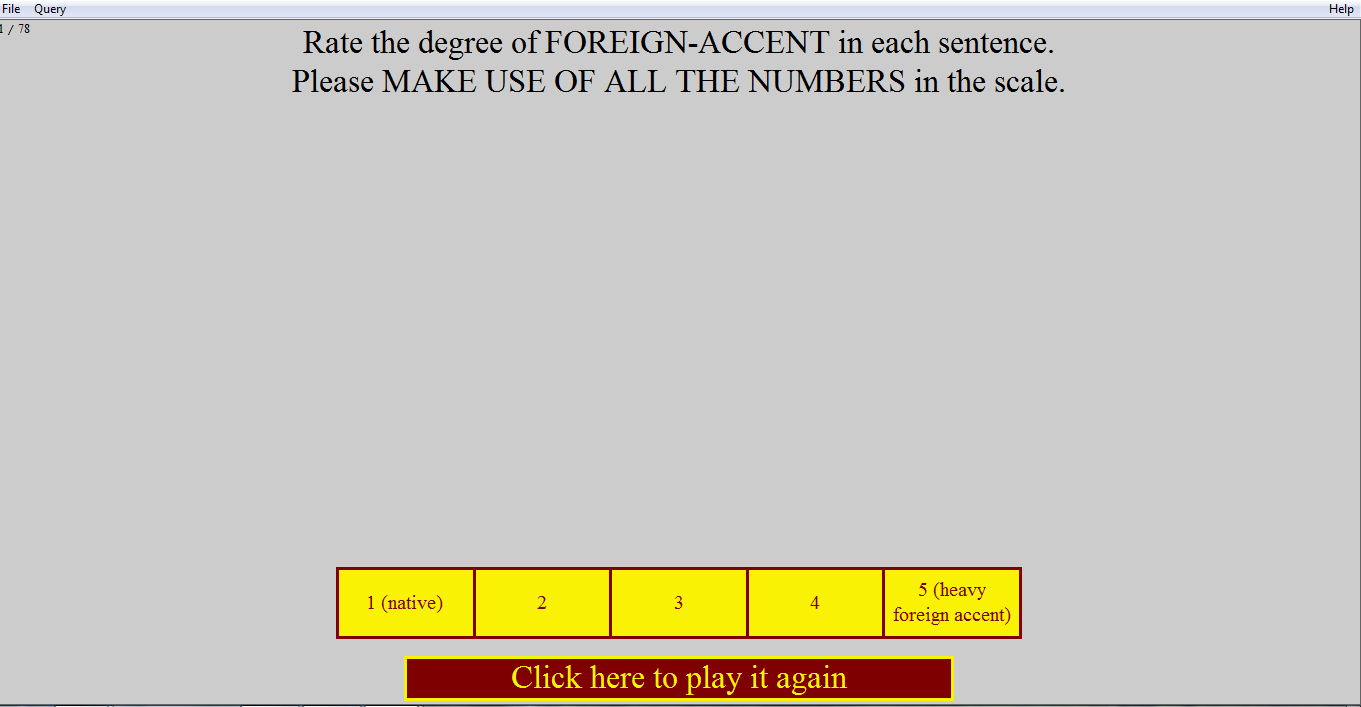
\includegraphics[width=\textwidth]{figures/avello-img1.png}
\end{figure}



A 9-point scale has been most commonly used in \isi{FA} studies, since participants usually differ greatly in \isi{proficiency} level, as well as in \isi{AOL} and/or \isi{L2} exposure. However, a 5-point scale was deemed more appropriate for the data in the present study, taking into account the smaller degree of variability in our oral samples (\isi{NNSs} with a similar age, \isi{AOL}, \isi{L2} exposure and \isi{proficiency} level).

Listeners were instructed to focus on \isi{pronunciation} and rate the degree of \isi{FA} they perceived in the speech samples as produced by the \isi{NNSs} and the \isi{NSs} by making use of the whole scale. Each stimulus was repeated twice for a total of 54 test trials per listener (8 \isi{NNSs} x 3 data collection times x 2 repetitions + 3 \isi{NSs} x 2 repetitions), resulting in a total of 702 ratings (54 trials x 13 listeners). Each listener heard the stimuli in a different randomized order. Listeners could replay each trial twice before providing their answer. After rating a stimulus, they had to click on a “next” button to listen to the following stimulus. If the \isi{NLs} made a mistake when rating a stimulus, they could click on an error button to listen to it again and change their answer (an answer could be changed only once). Listeners were presented with 16 practice trials (8 samples x 2 repetitions) before the test trials. During the test trials, there was the possibility of a pause after a block of 18 trials.


\section{Results}

Preliminary analyses were conducted to assess both intra-rater and inter-rater consistency in the \isi{NLs}’ ratings by means of Pearson correlations, which yielded both high intra-rater and inter-rater consistency coefficients. 

Regarding intra-rater reliability, there was a strong correlation in the listener-based \isi{FA} ratings assigned at each of the two rating repetitions (\textit{r} = .71, \textit{p} = .007), indicating that each listener’s first and second repetition ratings were strongly correlated; that is, each listener assigned similar ratings to the same stimulus at both the first and second repetitions.

Similarly, strong correlations were found in the stimulus-based \isi{FA} ratings assigned by the 13 listeners in all pair-wise combinations, with \textit{r} coefficients ranging between .74 and .98 (in all cases \textit{p} < .05), which indicates a high degree of agreement among listeners.

\tabref{tab:avello:1} and \figref{fig:avello:2} show the \isi{FA} ratings assigned by the \isi{NLs} to the baseline data provided by the \isi{NSs} (T0) and to the \isi{NNSs} through time (T1, T2 and T3). As expected, the ratings for the \isi{NSs} were very close to 1 (\textit{M} = 1.06), indicating that the listeners identified the \ili{English} \isi{NSs} and rated them accordingly. In contrast, the ratings assigned to the \isi{NNSs}’ were considerably outside the range of the \isi{NSs}’ ratings across all testing times. 

\begin{table}
\begin{tabularx}{\textwidth}{Xrrrrrr}
\lsptoprule
 Group &  Time &  \textit{n} &  Minimum &  Maximum &  Mean &  \textit{SD}\\
 \midrule
NS & T0 & 3 & 1.00 & 1.19 & 1.06 & .11\\
NNS & T1 & 8 & 2.58 & 4.58 & 3.19 & .68\\
~ & T2 & 8 & 2.62 & 4.23 & 3.47 & .49\\
~ & T3 & 8 & 3.04 & 3.81 & 3.40 & .31\\
\lspbottomrule
\end{tabularx}
\caption{\label{tab:avello:1}: Summary for FA ratings as assigned by the NLs (1 = native, 5 = heavy foreign accent)}
\end{table}


\begin{figure}
% 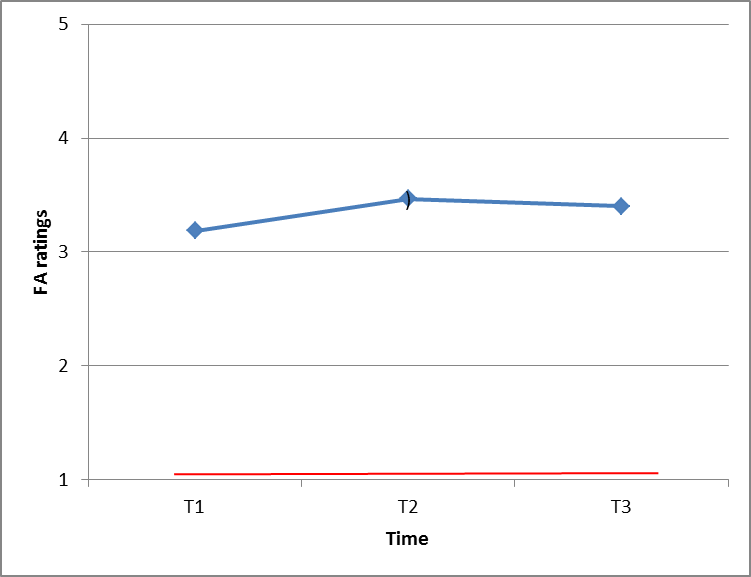
\includegraphics[width=\textwidth]{figures/avello-img2.png}
%  1.0641; 3,1875; 3,4663; 3,399
  \begin{tikzpicture}
    \begin{axis}[
	xlabel={Time},  
	ylabel={\isi{FA} ratings}, 
	axis lines*=left, 
        width  = .8\textwidth,
	height = .45\textheight,
    	nodes near coords, 
	xtick=data,
	x tick label style={}, 
	ymin=1,
	ymax=5,   
	symbolic x coords={T1,T2,T3},
	legend style={at={(1,0.4)},anchor=west}, 
	] 
	\addplot[draw=lsMidGreen,thick, dashed] 
	    coordinates {(T1,3.1875) (T2,3.4663) (T3,3.399) };
	\addplot[draw=lsDarkBlue,thick] 
	    coordinates {(T1,1.0641) (T2,1.0641) (T3,1.0641) };
% 	\legend{X, Y}
    \end{axis} 
  \end{tikzpicture} 
 
 
\caption{\label{fig:avello:2}: Mean FA ratings for the NSs (represented by the horizontal line) and the NNSs at T1 (at the beginning of the academic year), T2 (after an 80-hour FI period prior to SA) and T3 (upon return from a 3-month SA).}
\end{figure}


An increase in \isi{FA} ratings can be observed between T1 (\textit{M} = 3.19) and T2 (\textit{M} = 3.47), signaling no positive effect of \isi{FI} on the \isi{NNSs}’ degree of \isi{FA}. This is followed by a slight decrease in \isi{FA} ratings between T2 (\textit{M} = 3.47) and T3 (\textit{M} = 3.40), which seems to suggest a positive trend of improvement in the \isi{NNSs}’ degree of \isi{FA} during the SA period. A one-way repeated measures ANOVA was conducted with the \isi{FA} ratings as dependent variable and time as within-subjects factor in order to assess the effect of the \isi{FI} and SA learning contexts on the \isi{L2} learners’ \isi{pronunciation} development as measured by the \isi{FA} ratings. This analysis yielded a non-significant effect of time on the \isi{FA} ratings (Wilks’ Lambda = .64, \textit{F}(2, 6) = 1.69, \textit{p} = .26, \textit{$\eta $\textsuperscript{2} }= .36), indicating that the slight decrease observed in the \isi{FA} ratings as a result of SA failed to reach significance.\footnote{Results pooled across all listeners are presented, as the same results pattern was observed in the exchange students and \ili{English} teachers.}

Indeed, as illustrated in \tabref{tab:avello:1} and \figref{fig:avello:2}, the \isi{L2} learners’ \isi{FA} ratings remained similar through time. Independent samples \textit{t}{}-tests showed significant differences between the ratings assigned by the listeners to the \isi{NSs}’ and to the \isi{NNSs}’ at T1 (\textit{t}(9) = $-$5.21, \textit{p}  = .001, \textit{$\eta $\textsuperscript{2} }=  .75), T2 (\textit{t}(9) = $-$8.17, \textit{p} < .001, \textit{$\eta $\textsuperscript{2} }= .88), and T3 (\textit{t}(9) = $-$12.42, \textit{p} < .001, \textit{$\eta $\textsuperscript{2} }= .94). However, no significant differences were found between the three testing times for \isi{NNSs}, which indicates the lack of development toward NS patterns in terms of degree of \isi{FA}. Taken together, these results yield no evidence of significant improvement in \isi{FA} ratings during SA, although they seem to signal a positive trend of development toward less accented speech as a result of SA (as opposed to \isi{FI}). This suggests that SA might have had some impact on reducing the \isi{NNSs}’ degree of \isi{accentedness}, even though statistically non-significant.


\section{Discussion}

These results contrast with the findings reported in most studies assessing the effect of SA on \isi{L2} \isi{acquisition}. As noted in §2.2, SA has been generally found to have a clear positive impact on \isi{L2} \isi{linguistic} development, with results providing evidence of substantial SA gains in lexical development (\citealt{Collentine2004}; \citeauthor{LlanesMuñoz2009}), writing (\citealt{Sasaki2004}; \citealt{Pérez-VidalJuan-Garau2011}) and listening (\citealt{AllenHerron2003,LlanesMuñoz2009}). SA has been found to be particularly beneficial for the development of \isi{L2}
oral skills, such as overall oral \isi{proficiency}, enhanced accuracy and complexity, and most notably \isi{fluency} \citep{BrechtEtAl1995,SegalowitzFreed2004,FreedEtAl2004,Valls-Ferrer2011}. This is in line with the general assumption that \isi{oral production} is one of the areas that can be expected to improve the most during SA, as it is assumed to be one of the most practiced skills while abroad and to specially benefit from the massive exposure to \isi{L2} input that SA offers.

However, these results are consistent with the scant existing research analyzing SA gains in \isi{L2} \isi{pronunciation}, which has yielded inconclusive evidence regarding the effects of SA on this dimension. Whereas some studies have reported a positive effect of SA, for instance, on the production of consonantal segments \citep{Díaz-Campos2004,Díaz-Campos2006,Mora2008,SanzEtAl2013}, and rhythm metrics \citep{Valls-Ferrer2011}, other studies have failed to find substantial SA gains in \isi{vowel} production \citep{Simões1996,Avello2010a,Pérez-VidalEtAl2011}, and in the production of both \isi{vowel} and consonantal contrasts \citep{Højen2003}. \citet{Avello2010b} found that lack of improvement in \isi{vowel} contrast production following SA did not however prevent considerable gains in \isi{FA} scores. Conversely, results in \citet{AvelloEtAl2012} showed significant improvement in \isi{phonetic} measures of error rate scores during SA, whereas no significant improvement was found in \isi{FA} ratings. 

The lack of a stronger impact of SA on the \isi{FA} ratings attributed to \isi{L2} learners in the present study may be related to the length of the SA program. \isi{LoS} is one of the SA program features identified by \citet{Pérez-VidalJuan-Garau2011} as influencing SA outcomes, since it determines amount of exposure to \isi{L2} input. \isi{LoS} would thus be the SA equivalent to \isi{LOR}, which is the variable that has traditionally been used as an index for amount of exposure to \isi{L2} input in \isi{FA} studies analyzing the \isi{acquisition} of \isi{L2} speech within long-term, naturalistic \isi{immersion} contexts. 

In his study addressing \isi{FA} changes during SA by a group of L1 Danish undergraduate learners of \ili{English}, \cite{Højen2003} reported significant improvement in his participants’ \isi{FA} scores after their experience abroad. However, the participants in his study presented considerable variation in terms of \isi{LoS} in the SA context. The mean \isi{LoS} was 7.1 months (range = 3-11 months), which is considerably longer than the 3-month stay experienced by the learners in the present study. When analyzing these individual differences, Højen found a strong positive correlation between \isi{LoS} and gains in \isi{FA} scores (\textit{r} = .61, \textit{p} < .05). The learners who showed less improvement during SA were those with stays of only 3 to 4 months, which is in line with the results of the present study, whereas the greatest SA gains were obtained by the learners who stayed abroad up to 11 months. Højen interpreted these results as signaling the importance of \isi{LoS} for SA gains in \isi{FA} scores to accrue.

As indicated in §2.1 above, findings regarding the role of \isi{LOR} on degree of \isi{FA} in long-term \isi{immersion} contexts have been mixed, with some studies reporting an effect of \isi{LOR} on \isi{FA} ratings while other studies have failed to do so. The impact of \isi{LOR} seems to be influenced by \isi{L2} learners’ age and stage of \isi{L2} learning. \isi{LOR} seems to have an effect on \isi{L2} \isi{pronunciation} for early learners, but not for late or adult learners \citep{Flege1988}. It has been claimed that most \isi{L2} \isi{phonological} learning for late or adult \isi{L2} learners would take place within the first year of massive exposure in the \isi{L2} context. Pronunciation would then fossilize, resisting further changes after this initial period of gains (\citealt{Selinker1972,Flege1988,Scovel1988,FlegeFletcher1992}). More inexperienced late \isi{L2} learners (those at an early stage of \isi{L2} learning) could thus benefit from additional \isi{L2} exposure, whereas more experienced late \isi{L2} learners (those with higher \isi{proficiency}) would be unlikely to benefit from further \isi{L2} exposure.

The results reported in the present study could be interpreted in the light of these general findings for \isi{LOR} effects. Although the \isi{NNSs} in this study had been learning \ili{English} since childhood in \isi{FI} settings at their \isi{AH} institutions, opportunities for out-of-class exposure to conversational \ili{English} input are rather limited in Spain. The SA experience allowed them to live in an \ili{English}-speaking country and to have access to massive and authentic \isi{L2} \ili{English} input. However, as stated above, a 3-month \isi{LoS} might be too short to observe a significant improvement in these learners’ \isi{FA} ratings. Considering that there seemed to be a tendency toward a decrease in \isi{accentedness} during SA, it is possible that the \isi{NNSs}’ degree of \isi{FA} would have continued to gradually decrease with an increase in \isi{LoS} up to, for example, the average 7.1 months or 11 months at which significant improvement in \isi{FA} scores was reported by \cite{Højen2003}.

Improvement in \isi{FA} ratings seems to be further influenced by other factors, such as the actual amount and quality of the \isi{L2} input learners receive. According to \citet[197]{PiskeEtAl2001}, the inconclusive findings of research on \isi{LOR} effects can also be partly due to the fact that “\isi{LOR} only provides a rough index of overall \isi{L2} experience”. Following this line of thought, \citet{Højen2003} created a composite measure which weighted \isi{LoS} by self-reported \ili{English}-language input while abroad, and found that the correlation between this composite measure and gains in \isi{FA} scores (\textit{r} = .81, \textit{p} < .001) was stronger than the correlation between \isi{LoS} alone and gains in \isi{FA} scores as reported above. He interpreted this finding as an indication of the importance of having access to a substantial amount of high-quality \isi{L2} native input to improve \isi{FA} scores, in line with previous findings (\citealt{FlegeLiu2001}).

The learners in the present study reported a relatively high degree of contact with \ili{English} \isi{NSs} (an average of 3.6 on a 5-point scale, where 1 = ‘never’, 5 = ‘very often’), but they also reported a higher degree of contact with other \isi{NNSs} of \ili{English} (an average of 4.5 on the same scale). Since these learners were Erasmus students, it is very likely that they were in contact with other Erasmus students from a variety of non-\ili{English} speaking countries. Exposure to this poorer, foreign-accented \isi{L2} input could have thus contributed to the lack of significant improvement in their \isi{FA} ratings. In terms of accommodation, only one learner reported sharing an apartment with \ili{English} \isi{NSs}, whereas the rest reported staying in a single room at a residence hall. The fact that this was the preferred type of accommodation for the learners in this study might also have had some bearing on the lack of significant \isi{FA} gains, as this type of accommodation is more likely to limit opportunities for interaction with \isi{NSs} as compared with other options, such as sharing a room or apartment with \isi{NSs} or staying with a native family.

Another factor that has been found to influence \isi{FA} gains is learners’ patterns of L1 and \isi{L2} use during \isi{immersion} in the \isi{L2} context. Results reported in previous research suggest that more frequent use of the L1 (which would entail less frequent use of the \isi{L2}) is associated with higher degree of \isi{FA} \citep{FlegeEtAl1997,PiskeEtAl2001}. As is normally the case with Erasmus programs, the learners in the present study traveled to their SA destination in small groups and reported spending some time with the other students from their \isi{AH} university (an average of 1.5 on a 3-point scale, where 1 = ‘most time’, 3 = ‘little’). The learners further reported a rather high degree of contact with their families back home while abroad by means of a scale from ‘a’ to ‘e’ (‘a’ = ‘more than once a day’ and ‘e’ = ‘none’). Learners reported mostly ‘b’ (‘a few times a week’), indicating frequent contact, whereas none reported ‘d’ or ‘e’. These patterns of rather frequent L1 use could also have prevented the learners from obtaining greater gains in their \isi{FA} ratings.

The lack of greater changes in the learners’ \isi{FA} ratings could also be related to the way in which listeners process speech samples and how this influences their \isi{FA} ratings. Listeners seem to assess speech samples for overall degree of \isi{FA} holistically \citep{Magen1998}. This means that they pay attention to different speech features both at the segmental level (phonemic and subphonemic substitutions, insertions, deletions) and suprasegmental level (stress, pitch range, rhythm, speaking rate, connected speech phenomena, overall prosody, or \isi{intonation}), and that different listeners may also weigh these features of speech differently for different \isi{L2} learners and \isi{proficiency} levels. Some studies have reported a positive effect of a short SA program not exceeding 3 months on learners’ \isi{segmental production} (\citealt{Díaz-Campos2004,Díaz-Campos2006,Mora2008,SanzEtAl2013}). However, a 3-month SA program might not be long enough to trigger similar gains in other areas of \isi{pronunciation} involving prosodic features of speech, which have also been found to considerably bear on the perception of \isi{FA} (\citealt{Anderson-HsiehEtAl1992,MunroDerwing1999}).

Another factor which could have influenced the outcome of the \isi{FA} ratings is the rather homogeneous composition of the learner group in terms of \isi{L2} \isi{proficiency} level. Although there were differences in \isi{pronunciation} between the learners, they all shared a similar L1 background and \isi{L2} \ili{English} language level (B2 or upper-intermediate). This could have made the rating task rather difficult for the listeners, who had to discriminate subtle \isi{FA} changes between learners and across testing time. It is probably easier for listeners to rate speech samples from a pool of learners showing a wider range of \isi{proficiency} levels, from low to advanced. This has typically been the case in the \isi{FA} literature examining long-term \isi{immersion} contexts, where differences in \isi{FA} scores arise as a result of considerable inter-subject variation in terms of \isi{L2} \isi{proficiency}, which in turn can be attributed to differences in \isi{AOL}, as well as to other variables such as \isi{L2} exposure, L1/\isi{L2} use, etc. (see §2.1). It is also possible that the use of a scale wider than the 5-point scale used in the present study would have better captured the slight changes in \isi{pronunciation} that the learners might have experienced.  


\section{Conclusion}

To sum up, results in the present study showed no improvement in the \isi{NNSs}’ \isi{FA} ratings as a result of \isi{FI} and suggested, in contrast, a positive trend of development toward a decrease in \isi{FA} following SA, although this decrease was not significant and the \isi{NNSs}’ \isi{FA} ratings remained significantly different from the \isi{NSs}’ \isi{FA} ratings through time. This outcome is in line with the mixed results that have been reported in the scarce research that has assessed the effect of SA as compared with \isi{FI} on \isi{L2} \isi{pronunciation}. Given the observed trend of development during SA, maybe an increased \isi{LoS} could have resulted in continued gradual improvement leading to significant gains in the \isi{NNSs}’ \isi{FA} ratings, as is suggested in previous research \cite{Højen2003}. Since general findings from research on \isi{L2} \isi{speech production} suggest that most progress in \isi{pronunciation} takes place during the first year of \isi{immersion} in an \isi{L2} context, more studies are needed focusing on the effects of \isi{LoS} on \isi{pronunciation} outcomes for \isi{L2} learners with different \isi{proficiency} levels. 

Considering the holistic way in which listeners provide \isi{FA} ratings, and the fact that different listeners may focus on different aspects of \isi{L2} speech, it is also possible that the \isi{FA} ratings in the present study failed to reflect some gains that could have accrued in some specific features of the learners’ \isi{L2} \isi{pronunciation}. Such changes could have been captured by fine-grained \isi{phonetic} or acoustic analyses, or could have been reflected in the \isi{FA} ratings by means of the use of a scale with a wider range. Previous research has found that the relation between \isi{FA} ratings and specific aspects of \isi{pronunciation} is not always a straightforward one. For example, \citet{AvelloEtAl2012} found significant SA gains in \isi{phonetic} error rate scores, but not in \isi{FA} scores. Conversely, in \citet[237]{RineyFlege1998}, gains in global \isi{FA} ratings did not coincide with improvement in \isi{segmental production} regarding liquid identifiability and accuracy. The authors noted that it “appears not to be the case that improvement in global \isi{accent} necessarily proceeds in parallel with improvement in any particular smaller components of \isi{pronunciation}, such as segmental identifiability and accuracy”. In this sense, in order to gain better insight into the types of changes that can be expected in \isi{L2} \isi{pronunciation} as a result of SA, more research is needed with a multiple-measures approach that combines subjective \isi{FA} scores as well as more objective acoustic and \isi{phonetic} analyses that include acoustic measures and error rate scores.

\section*{Acknowledgements}

This research was funded by grant FFI2010-21483-C02-01 awarded by the \ili{Spanish} Government to the SALA project, and by grants BES-2008-010037 and EEBB-I-12-04294 awarded by the \ili{Spanish} Government to the author within the FPI doctoral research program.

 
\sloppy
\printbibliography[heading=subbibliography,notkeyword=this] 
\end{document}